\documentclass[10pt,landscape]{article}
\usepackage{multicol}
\usepackage{calc}
\usepackage{ifthen}
\usepackage[landscape]{geometry}
\usepackage{amsmath,amsthm,amsfonts,amssymb}
\usepackage{color,graphicx,overpic}
\usepackage{tikz}
\usepackage{tikz-3dplot}
\usepackage{pgfplots}
\usetikzlibrary{shapes.geometric}
\usetikzlibrary{decorations.markings}



\pdfinfo{
  /Title (Biochem.pdf)
  /Creator (TeX)
  /Producer (pdfTeX 1.40.0)
  /Author (Kevin)
  /Subject (Biochemistry Cheat Sheet)
  /Keywords (biochemistry, tex, latex)}

\geometry{top=.5in,left=.5in,right=.5in,bottom=.5in}

% Turn off header and footer
\pagestyle{empty}

% Redefine section commands to use less space
\makeatletter
\renewcommand{\section}{\@startsection{section}{1}{0mm}%
                                {-1ex plus -.5ex minus -.2ex}%
                                {0.5ex plus .2ex}%
                                {\normalfont\large\bfseries}}
\renewcommand{\subsection}{\@startsection{subsection}{2}{0mm}%
                                {-1explus -.5ex minus -.2ex}%
                                {0.5ex plus .2ex}%
                                {\normalfont\normalsize\textit}}
\renewcommand{\subsubsection}{\@startsection{subsubsection}{3}{0mm}%
                                {-1ex plus -.5ex minus -.2ex}%
                                {1ex plus .2ex}%
                                {\normalfont\small\underline}}
\makeatother

\renewcommand{\baselinestretch}{1.5}

% Don't print section numbers
\setcounter{secnumdepth}{0}


\setlength{\parindent}{0pt}
\setlength{\parskip}{0pt plus 0.5ex}

%My Environments
\newtheorem{example}[section]{Example}
%

\pgfplotsset{width=6cm,compat=1.9}


\begin{document}
\raggedright
\footnotesize
\begin{multicols}{3}


% multicol parameters
% These lengths are set only within the two main columns
%\setlength{\columnseprule}{0.25pt}
\setlength{\premulticols}{1pt}
\setlength{\postmulticols}{1pt}
\setlength{\multicolsep}{1pt}
\setlength{\columnsep}{2pt}

\begin{center}
     \Large{\textbf{Biochemistry}} \\
\end{center}

\section{Proteins}
\subsection{Isoelctric Point}
Average pKa of the zwitterion: $\text{pi}=\dfrac{pKa1*pKa2}{2}$

\section{Enzymes}
\subsection{Overview}
$\cdot$ Active site vs Induced fit model: In the former the active site matches the substrate while in the former the substrate slightly temporarily alters the active site creating a better fit \newline
$\cdot$ Co-Enzyme: Organic carrier molecules \newline
$\cdot$ Enzyme cofactor  is a an inorganic molecule that is nessecary for an enzyme to function \newline
$\cdot$ Vitamins and Minerals: The former being organic and the latter being inorganic and both of which not being produced naturally and are often used as co-factors and co-enzymes

\subsection{Catalytic Strategies}
$\cdot$ Acid/Base \newline
$\cdot$ Covalent \newline
$\cdot$ Electrostatic \newline
$\cdot$ Proximity/Orientation \newline

\subsection{Types}
$\cdot$ Transferase: Transfers a functional group from A to B \newline
$\cdot$ Ligase: Joins together A and B through dehydration reaction \newline
$\cdot$ Oxidoreductase: Assist w/ a redox reaction \newline
$\cdot$ Isomerase: Converts a molecule to one of its isomers \newline
$\cdot$ Hydrolase: Breaks molecule in two parts through hydrolysis  \newline
$\cdot$ Lyase: Breaks molecule without using hydrolysis or redox typically using double bonds \newline

\section{Enzyme Kinetics}
\subsection{Michaelis-Menten and Lineweaver Burke}
\subsubsection{Values}
$V_{max}$: Fastest speed for a given Enzyme and substrate \newline
$K_{M}$ is the $[S]$ where $\dfrac{1}{2}V_{max}$ is achieved \newline
$k_{cat}$: Turnover rate \newline

\subsubsection{Relations}
$K_{M}$ is the $[S]$ where $\dfrac{1}{2}V_{max}$ is achieved \newline
Catalytic Efficiency = $\dfrac{k_{cat}}{K_{M}}$ \newline
$V_{max}=k_{cat}[E]$ \newline
$K_{M} \propto$ Substrates affinity of an enzyme \newline

\subsubsection{Michaelis-Menten}
$V_{0}= \dfrac{V_{max}[S]}{k_{m}+[S]}$ \newline

\begin{tikzpicture}
\begin{axis}[
    axis lines = left,
    xlabel = {$[S]$},
    ylabel = {$V_{0}$},
    yticklabels={,,},
    xticklabels={,,}
]
\addplot[
	color=red,
    domain=0:5, 
    samples=100, 
    color=red,
    ]
{(3*x)/(0.5+x)};
\end{axis}
\end{tikzpicture}

\subsubsection{Lineweaver-Burk}
$\dfrac{1}{V_{0}}=\dfrac{k_{m}}{V_{max}[S]}+\dfrac{1}{V_{max}}$ \newline

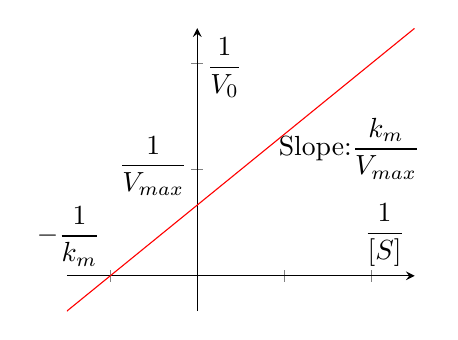
\begin{tikzpicture}
\begin{axis}[
    axis lines = center,
    clip mode=individual,
    xlabel = {$\dfrac{1}{[S]}$},
    ylabel = {$\dfrac{1}{V_{0}}$},
    clip mode = individual,
    yticklabels={,,},
    xticklabels={,,}
]
\addplot[
	color=red,
    domain=-3:5, 
    samples=100, 
    color=red,
    ]
{((0.5)/3*x)+(1/3)};
\node[above left] at (axis cs:0,0.33) {$\dfrac{1}{V_{max}}$};
\node[above left] at (axis cs:-2,0) {$-\dfrac{1}{k_{m}}$};
\node at (axis cs:3.5,0.6) {Slope:$\dfrac{k_{m}}{V_{max}}$};
\end{axis}
\end{tikzpicture}


\subsection{Enzyme Inhibition}
Competitive Inhibitor: Binds to [E]
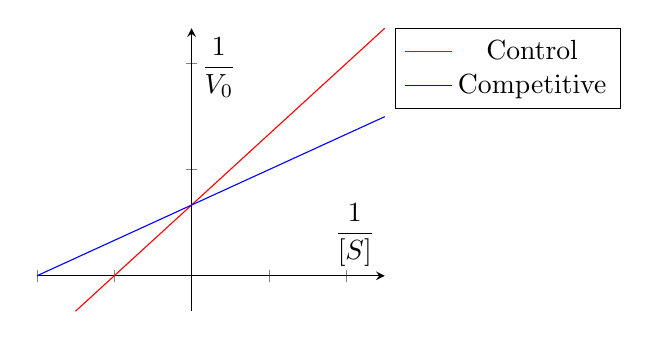
\begin{tikzpicture}
\begin{axis}[
    axis lines = center,
    clip mode=individual,
    xlabel = {$\dfrac{1}{[S]}$},
    ylabel = {$\dfrac{1}{V_{0}}$},
    clip mode = individual,
    yticklabels={,,},
    xticklabels={,,},
    legend pos= outer north east
]
\addplot[
    domain=-3:5, 
    samples=100, 
    color=red,
    ]
{((0.5)/3*x)+(1/3)};
\addlegendentry{Control}
\addplot[
    domain=-4:5, 
    samples=100, 
    color=blue,
    ]
{((0.25)/3*x)+(1/3)};
\addlegendentry{Competitive}
\end{axis}
\end{tikzpicture}
\newline

Non-Competitive Inhibitor: Binds to [E] + [ES]
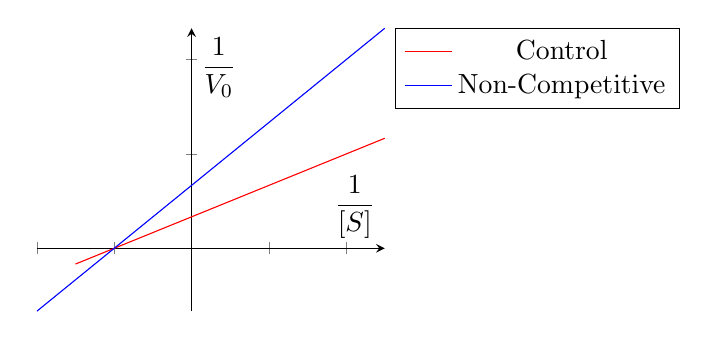
\begin{tikzpicture}
\begin{axis}[
    axis lines = center,
    clip mode=individual,
    xlabel = {$\dfrac{1}{[S]}$},
    ylabel = {$\dfrac{1}{V_{0}}$},
    clip mode = individual,
    yticklabels={,,},
    xticklabels={,,},
    legend pos= outer north east
]
\addplot[
    domain=-3:5, 
    samples=100, 
    color=red,
    ]
{((0.5)/3*x)+(1/3)};
\addlegendentry{Control}
\addplot[
    domain=-4:5, 
    samples=100, 
    color=blue,
    ]
{((0.5)/1.5*x)+(1/1.5)};
\addlegendentry{Non-Competitive}
\end{axis}
\end{tikzpicture}
\newline

Un-Competitive Inhibitor: Binds to [ES]
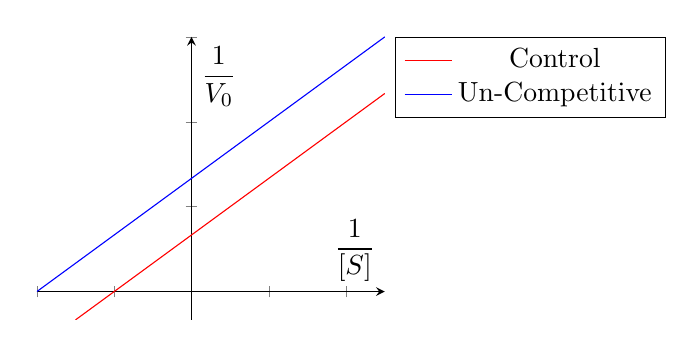
\begin{tikzpicture}
\begin{axis}[
    axis lines = center,
    clip mode=individual,
    xlabel = {$\dfrac{1}{[S]}$},
    ylabel = {$\dfrac{1}{V_{0}}$},
    clip mode = individual,
    yticklabels={,,},
    xticklabels={,,},
    legend pos= outer north east
]
\addplot[
    domain=-3:5, 
    samples=100, 
    color=red,
    ]
{((0.5)/3*x)+(1/3)};
\addlegendentry{Control}
\addplot[
    domain=-4:5, 
    samples=100, 
    color=blue,
    ]
{((0.25)/1.5*x)+(1/1.5)};
\addlegendentry{Un-Competitive}
\end{axis}
\end{tikzpicture}

\subsection{Cooperativity}
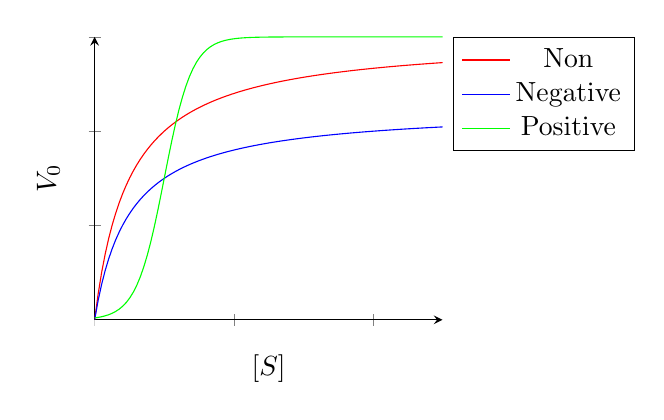
\begin{tikzpicture}
\begin{axis}[
    legend pos= outer north east,
    axis lines = left,
    xlabel = {$[S]$},
    ylabel = {$V_{0}$},
    yticklabels={,,},
    xticklabels={,,}
]
\addplot[
	color=red,
    domain=0:5, 
    samples=100, 
    color=red,
    ]
{(3*x)/(0.5+x)};
\addlegendentry{Non}
\addplot[
	color=blue,
    domain=0:5, 
    samples=100, 
    ]
{0.75*(3*x)/(0.5+x)};
\addlegendentry{Negative}
\addplot[
	color=green,
    domain=0:5, 
    samples=100, 
    ]
{3/(1+2.7182^(5-5*x))};
\addlegendentry{Positive}
\end{axis}
\end{tikzpicture}

\subsection{Allosteric Regulation}
Activator: $\uparrow$ Vmax and $\downarrow$ Km \newline
Inhibitor: $\downarrow$ Vmax and $\uparrow$ Km \newline
Homotropic Regulator: Same as the substrate \newline
Heterotropic Regulator: Different than the substrate \newline

\subsection{Enzyme Modification}
\subsubsection{Types}
Methylation: Adding a methyl group \newline
Acetylation: Adding an acetyl group \newline
Glycosylation: Adding a sugar  \newline
Suicide Inhibitors utilize covalent modification to irriversably bind to an enzyme

\subsubsection{Zymogens}
$\cdot$ Inactive enzyme that require chemical modification \newline
$\cdot$ Enzymes of this type end in -ogen \newline
$\cdot$ Often used in digestive system to avoid breaking down in wrong location \newline


\end{multicols}
\end{document}